\section{Team structure}
\subsection{About}
Our team is mainly composed of INSA Lyon students, with the exception of students from
\begin{itemize}
    \item INSA Strasbourg
    \item \todo{Julie} IUT Lyon 1
    \item \todo{Oliver}.
\end{itemize}
The teams operate in English, due to the significant number of international members.

\subsection{Organization}
Our club's main leaders are Paul Retourné (FX27 lead), Yaroslav Knyazkov (Mechanical lead), and Issam Kerrouche (Electrical lead).

The Fusex project is split into an electrical team and a mechanical team, with the mechanical team further subdivided into systems.
Each team is run by a team lead, and team meetings are held weekly.
Tasks are tracked in a shared spreadsheet and divided by team, as shown in figure \ref{fig:team-structure}.
We are in the process of developing a spreadsheet for variable management and an inquiry system, where one team can request a parameter from another team.

\begin{figure}[ht]
    \centering
    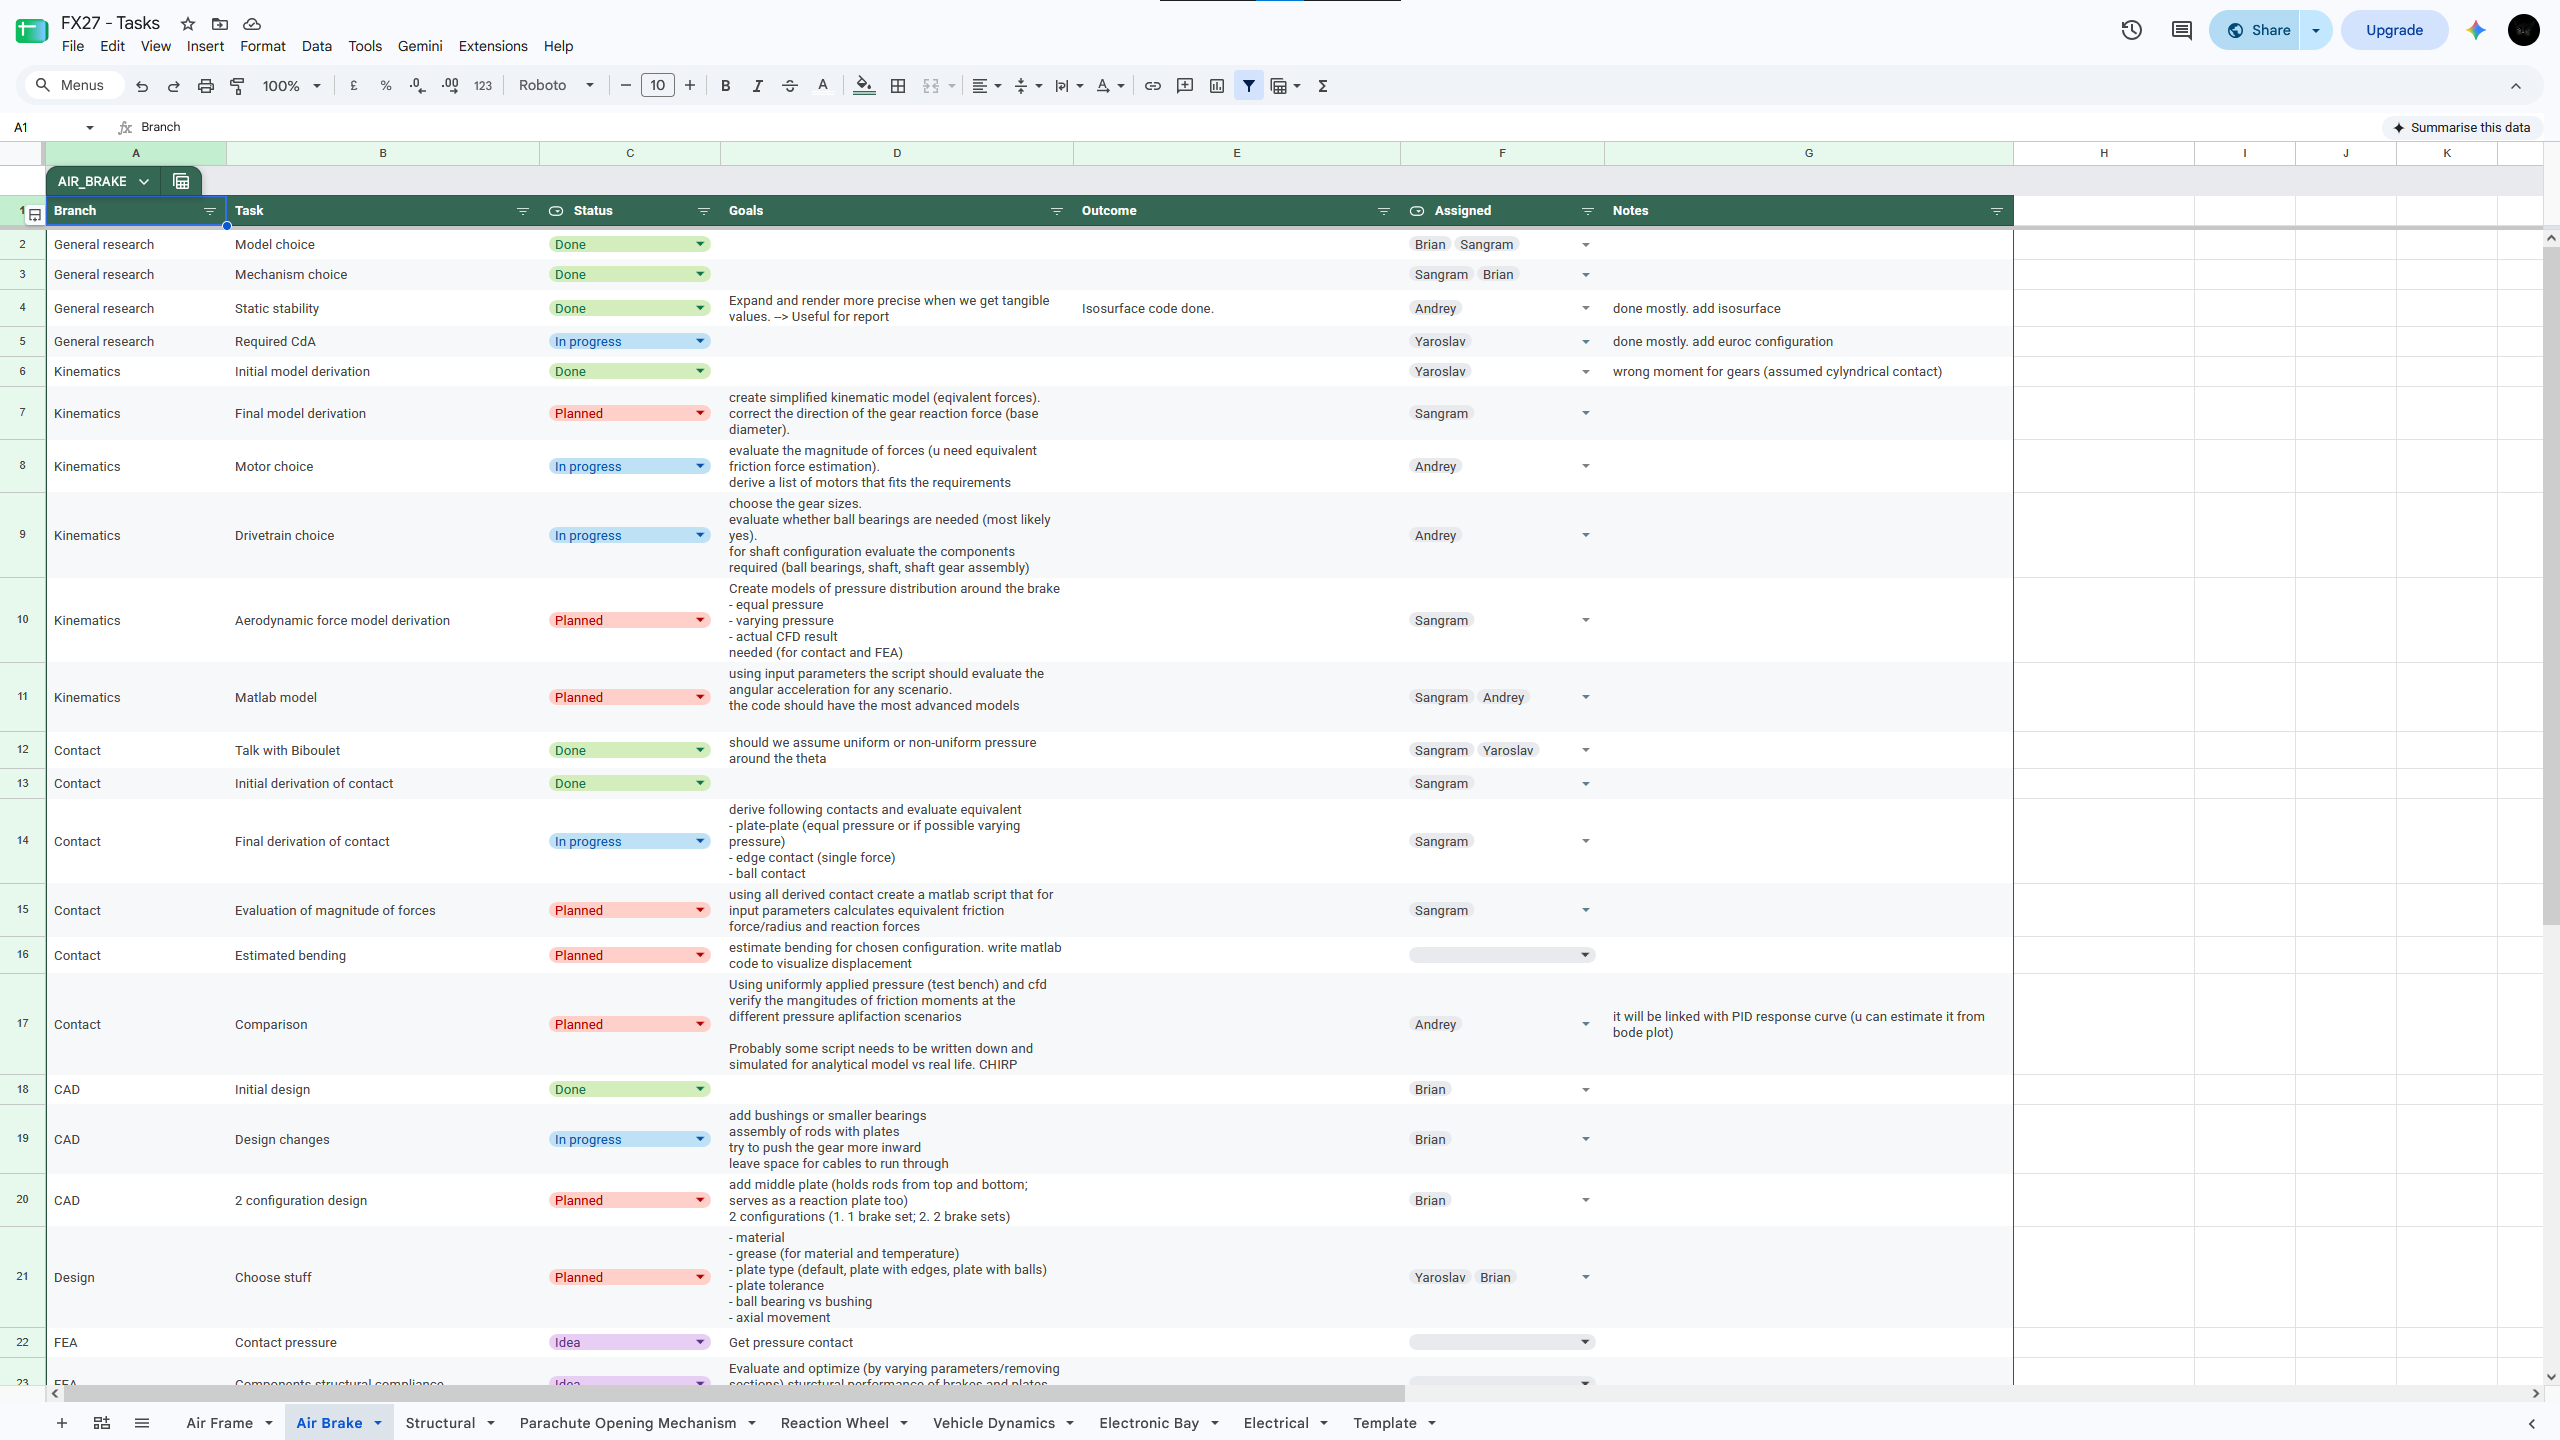
\includegraphics[width=\textwidth]{Tasks.png}
    \caption{Team structure and task breakdown.}
    \label{fig:team-structure}
\end{figure}